%############################################################################
\section{Two-Step Verification}
\label{sec:m-twostep}
%############################################################################

Two-step verification builds on the methods presented before, combining them to produce improved user feedback.

Implicit contracts are simply added whenever appropriate and used to have early detection of errors violating them.
In AutoProof, which translates Eiffel to Boogie to perform static proofs, implicit contracts are not added to the Eiffel code but are silently injected into the Boogie translation, so that the input code does not become polluted by many small assertions; users familiar with Eiffel's semantics are aware of them without explicitly writing them down.
Errors consisting of violations to implicit contracts reference back the original statements in Eiffel code from which they originated, so that the error report is understandable without looking at the Boogie translation.

Whenever the verifier checks a routine that contains routine calls, two-step verification applies inlining as described in Section~\ref{sec:with-inlining}.
Whenever it checks a routine that contains loops, two-step verification applies unrolling as described in Section~\ref{sec:with-unrolling}.
The application of the two steps is completely automatic, and is combined for routines that includes both calls and loops; users only get a final improved error report in the form of suggestions that narrow down the possible causes of failed verification more precisely than in standard approaches.
Section~\ref{sec:examples-two-step} briefly illustrates two-step verification on the running example of Section~\ref{sec:ap-overview}.






%============================================================================
\subsection{With Inlining}\label{sec:with-inlining}
%============================================================================

Consider a generic routine \e{r} with precondition $P_r$ and postcondition $Q_r$, whose body $B_r$ contains a call \e{t.s(a)} to another routine \e{s} with precondition $P_s$, postcondition $Q_s$ and body $B_s$ (as shown in Figure~\ref{r-calls-s}).
Two-step verification runs two verification attempts on $r$:
\begin{enumerate}
\item \textbf{Modular verification:} The first step of two-step verification for $r$ follows the standard modular verification approach: it tries to verify that $r$ is correct with respect to its specification, using $s$'s specification only to reason about the call to $s$; and then it separately tries to verify $s$ against its own specification.

\item \textbf{Inlined verification:} The second step of two-step verification for $r$ replaces the call to $s$ in $r$ with $\inline(t.s(a), n)$, for some $n > 0$ picked as explained in Section~\ref{sec:bounds}, and then verifies $r$ with this inlining.
\end{enumerate}

\begin{figure}[!tbh]
\centering
\begin{tabular}{lll}
{\begin{erunning}
r
  require $P_r$
  do
    $B_r \ \left\{\begin{array}{c}
        \vdots \\
        t.s (a)  \\
        \vdots
     \end{array}\right.
     $
   ensure $Q_r$
\end{erunning}}
&
$\qquad\quad$
{\begin{erunning}
s
  require $P_s$
  do
    $B_s$
  ensure $Q_s$
\end{erunning}}
&
$\qquad$
{\begin{erunning}
q
  require $P_q$
  do
    $\vdots$
    $L \ \left\{ \begin{array}{l}
    \textbf{until} \ e \\
    \textbf{invariant} \ I \\
    \textbf{loop} \ B \\
    \textbf{variant} \ V\ \textbf{end}
    \end{array} \right. $
    $\vdots$
  ensure $Q_q$
\end{erunning}}
\end{tabular}
\caption{A routine \e{r} calling another routine \e{s}; and a routine \e{q} with a loop.} \label{r-calls-s}
\end{figure}

\begin{table}[!tbh]
\centering
%\setlength{\tabcolsep}{5pt}
\begin{tabular}{cc c l}
\multicolumn{2}{c}{\textbf{step 1: modular}}  & \multicolumn{1}{c}{\textbf{step 2: inlined}}  & \\
\textsc{verify} $r$  &  \textsc{verify} $s$  &  \textsc{verify} $r$ & \textsc{suggestion} \\
\hline
\textcolor{darkred}{$P_s$ fails}  &  \textcolor{darkgreen}{success}  &  \textcolor{darkgreen}{success}  & weaken $P_s$ or use inlined \e{s} \\
\textcolor{darkred}{$Q_r$ fails}  &  \textcolor{darkgreen}{success}  &  \textcolor{darkgreen}{success}  & strengthen $Q_s$ or use inlined \e{s} \\
\textcolor{darkgreen}{success}  &  \textcolor{darkred}{$Q_s$ fails}  &  \textcolor{darkgreen}{success}  & strengthen $P_s$ or weaken $Q_s$
\end{tabular}
  \caption{Two-step verification with inlining: summary of suggestions.}
  \label{tab:two-step-inline-summary}
\end{table}


Each of the two steps may fail or succeed.
According to the combined outcome, we report a different suggestion to users, as summarized in Table~\ref{tab:two-step-inline-summary}.

%----------------------------------------------------------------------------
\subsubsection{Precondition fails}
%----------------------------------------------------------------------------

If modular verification (first step) fails to establish that $s$'s precondition $P_s$ holds right before the call, but both modular verification of $s$ and inlined verification (second step) of $r$ succeed, it means that $s$'s precondition may be inadequate\footnote{As with all failed static verification attempts, we cannot exclude that failure is simply due to limitations of the theorem prover.} while its implementation is correct with respect to its specification and to the usage made within $r$.
In this case, there are two options: if $s$ is a helper function used only in $r$ or inside a single class, we may as well drop $s$'s specification and just use it inlined wherever needed during verification.
In more general cases, we should try to \emph{weaken} $P_s$ in a way that better characterizes the actual requirements of how $s$ is used.

%----------------------------------------------------------------------------
\subsubsection{Postcondition fails}
%----------------------------------------------------------------------------

If modular verification fails to establish that $r$'s postcondition $Q_r$ holds when $B_r$ terminates, but both modular verification of $s$ and inlined verification of $r$ succeed, it means that $s$'s postcondition fails to characterize $r$'s requirements while $s$'s  implementation is correct with respect to its specification.
As in the previous case, there are two options: we may drop $s$'s specification and just use it inlined; or we should try to \emph{strengthen} $Q_s$ in a way that better characterizes the actual expectations of $r$ on $s$.
A similar scheme applies not just to failed postconditions $Q_r$  but whenever modular verification fails to verify intermediate assertions occurring on paths after the call to $s$ in $r$.


%----------------------------------------------------------------------------
\subsubsection{Local proof fails}
%----------------------------------------------------------------------------

If modular verification fails to establish that $s$'s postcondition $Q_s$ holds when $B_s$ terminates, but both modular verification of $r$ and inlined verification of $r$ succeed, it means that $s$'s specification cannot be proved consistent with its implementation, while the latter  is correct with respect to the usage made within $r$.
The suggestion is to change $s$ specification in a way that still accommodates its usage within $r$ and can be verified: strengthen the precondition $P_s$, weaken the postcondition $Q_s$, or both.
With this information, there is no way to decide if the problem is with the pre- or postcondition, but we can always try to modify either one and run verification again to see if the suggestion changes.


%----------------------------------------------------------------------------
\subsubsection{Other cases}
%----------------------------------------------------------------------------

In the remaining cases, two-step verification is inconclusive in the sense that it gives the same feedback as modular verification alone.
In particular, when the second step fails it is of no help to determine whether the problem is in the specification or the implementation.
If, for example, both modular and inlined verification of $r$ fail to establish the postcondition $Q_r$, but modular verification of $s$ succeeds, we cannot conclude that $s$'s implementation is wrong because it does not achieve $Q_r$: it may as well be that $r$'s implementation is wrong, or $r$'s postcondition is unreasonable; which is exactly the information carried by a failed modular verification attempt.

Also notice that inlined verification cannot fail when modular verification fully succeeds: if $s$'s implementation satisfies its specification, and that specification is sufficient to prove $r$ correct, then the semantics of $s$ within $r$ is sufficient to prove the latter correct.
Therefore, we need not run the second step when the first one is successful.\footnote{Again, exceptions might occur due to shortcomings of the theorem prover used by the modular verifier, which might be able to prove a set of verification conditions but fail on a syntactically different but semantically equivalent set due to heuristics or limitations of the implementation. These are, however, orthogonal concerns.}





%============================================================================
\subsection{With Unrolling} \label{sec:with-unrolling}
%============================================================================

Consider a generic routine $q$ with precondition $P_q$ and postcondition $Q_q$, whose body $B_q$ contains a loop $L$ with exit condition $e$, invariant $I$, variant $V$, and body $B$ (as shown in Figure~\ref{r-calls-s}).
Two-step verification runs two verification attempts on $r$:

\begin{enumerate}
\item \textbf{Modular verification:} The first step of two-step verification for $r$ follows the standard modular verification approach: it tries to verify that $r$ is correct with respect to its specification, using the loop invariant $I$ only to reason about the effect of $L$ within $r$; and then it separately tries to verify that $I$ is a correct inductive loop invariant (that is, it holds on entry and is maintained by iterations of the loop).

\item \textbf{Unrolled verification:} The second step of two-step verification for $r$ replaces the loop $L$ in $r$ with $\unroll(L, n)$, for some $n > 0$ picked as explained in Section~\ref{sec:bounds}, and then verifies $r$ with this unrolling and the additional assertion \e{assert V <= n}, evaluated upon loop entry, that the loop executes at most $n$ times.\footnote{If a variant is not available or cannot be verified to be a valid variant, we proceed as if the assertion did not hold.}
\end{enumerate}

\begin{table}[!tbh]
\centering
\setlength{\tabcolsep}{4pt}
\begin{tabular}{c cc l}
\multicolumn{1}{c}{\textbf{step 1: modular}}  & \multicolumn{2}{c}{\textbf{step 2: unrolled}}  & \\
\textsc{verify} $r$  & \e{assert V <= $\,$n}  & \textsc{verify} $r$ & \textsc{suggestion} \\
\hline
\textcolor{darkred}{$Q_q$ fails}  &  \textcolor{darkgreen}{success} &  \textcolor{darkgreen}{success}  &  use inlined $L$ \\
\textcolor{darkred}{$Q_q$ fails}  &  \textcolor{darkred}{fail} &  \textcolor{darkgreen}{success}  &  strengthen $I$ to generalize \\
\textcolor{darkred}{$I$ fails inductiveness}  &  \textcolor{darkgreen}{success} &  \textcolor{darkgreen}{success}  &  use inlined $L$ \\
\textcolor{darkred}{$I$ fails inductiveness} &  \textcolor{darkred}{fail} &  \textcolor{darkgreen}{success}  &  change $I$ to generalize \\
\end{tabular}
  \caption{Two-step verification with unrolling: summary of suggestions.}
  \label{tab:two-step-unroll-summary}
\end{table}

Each of the two steps may fail or succeed.
According to the combined outcome, we report a different suggestion to users, as summarized in Table~\ref{tab:two-step-unroll-summary}.

%----------------------------------------------------------------------------
\subsubsection{Postcondition fails}
%----------------------------------------------------------------------------

Suppose that modular verification (first step) fails to establish that $r$'s postcondition $Q_q$ holds when $B_q$ terminates, but unrolled verification (second step) of $r$ succeeds.
The suggestion in this case depends on whether the prover can also establish the intermediate assertion \e{assert V <= n}.
If it does, $n$ is a finite upper bound on the number of loop iterations in every execution.
Thus, the loop implementation is correct but the loop invariant $I$ is inadequate to prove the postcondition; we may as well drop the invariant $I$ and just use the exhaustively unrolled loop during verification.
In the more general case where the assertion \e{V <= n} fails, the successful unrolled proof shows that the loop body works with a finite number of iterations, and hence it is likely correct; we may then try to strengthen (or otherwise change) the invariant $I$ in a way that captures a generic number of loop iterations and is sufficiently strong to establish $Q_q$.
A similar scheme applies not just to failed postconditions $Q_q$ but whenever modular verification fails to verify intermediate assertions occurring on paths after the loop $L$ in $q$.


%----------------------------------------------------------------------------
\subsubsection{Invariant fails}
%----------------------------------------------------------------------------

Suppose that modular verification fails to establish that $I$ is inductive, but unrolled verification of $r$ succeeds.
The suggestion depends on whether the prover can also establish the intermediate assertion \e{assert V <= n}.
If it does, the loop implementation is correct but the loop invariant $I$ is inadequate; we may as well drop the invariant $I$ and just use the exhaustively unrolled loop during verification.
In the more general case where the assertion \e{V <= n} fails, the successful unrolled proof shows that the loop body works with a finite number of iterations, and hence it is likely correct; we may then try to change the invariant $I$ in a way that captures a generic number of loop iterations and is sufficiently strong to establish $Q_q$.
With this information, there is no way to decide if the invariant should be strengthened or weakened, but we can always try either one and run verification again.

In the remaining cases, two-step verification gives the same feedback as modular verification alone.
And, as for inlining, we need not run the second step (unrolled verification) when modular verification is completely successful.



%============================================================================
\subsection{Bounds for Nesting and Loops} \label{sec:bounds}
%============================================================================

The application of inlining and unrolling requires a parameter $n$: the maximum depth of nested calls in the former case; and the number of explicit iterations of the loop in the latter.
The choice of $n$ is more subtle for unrolling---where it should represent a number of iterations sufficient to make the second step of verification succeed---than for inlining---where it becomes relevant only in the presence of nested calls or recursion.

We use simple heuristics to pick values for $n$ that are ``feasible'', that is do not incur combinatorial explosion.
In the case of inlining, we get a crude estimate of the size of the inlined program as follows.
For a routine $p$, let $\paths_p$ denote the total number of simple paths in $p$ from entry to exit.
If $p$ has size $|p|$ (measured in number of instructions) and includes $m$ calls to routines $r_1, \ldots, r_m$, we recursively define $\insize{p}_n$ as: $|p|$ if $n = 0$,  $|p| + \paths_p (\insize{r_1}_{n-1} + \cdots + \insize{r_m}_{n-1})$ if $n > 0$.
The value of $\insize{p}$ is an upper bound to the total number of instructions on all possible paths of the inlined routine.
Inlining in $p$ uses an $n$ such that $\insize{p}_n \leq 10^4$.
In the case of unrolling a loop within routine $q$, our implementation does some simple static analysis to determine if the calling context of $q$ or $q$'s precondition suggest a finite bound of the loop (in practice, this is restricted to loops over arrays that are declared statically or with a constant upper bound in the precondition).
In such cases, $n$ is simply the inferred bound.
Otherwise, we roughly estimate the size of an unrolled loop $L$ as $n|L|$, where $|L|$ is the size of $L$ in number of instructions; unrolling $L$ uses an $n$ such that $n|L| \leq 10^3$.

In many practical cases (in the absence of recursion or deeply nested calls), very small $n$'s (such as $1 \leq n \leq 5$) are sufficient to produce a meaningful results in two-step verification.




%============================================================================
\subsection{Examples} \label{sec:examples-two-step}
%============================================================================

Let us demonstrate how two-step verification works on the examples introduced in Section~\ref{sec:ap-overview}.
Figure~\ref{ex:twowaysort-client} shows two clients of routine \e{two_way_sort} (Figure~\ref{ex:twowaysort}).
Routine \e{client_1} calls \e{two_way_sort} on an empty array, which is forbidden by \e{two_way_sort}'s precondition.
Normally, this is blamed on \e{client_1}; with two-step verification, however, the second verification attempt inlines \e{two_way_sort} within \mbox{\e{client_1}} and successfully verifies it.
This suggests that \e{client_1} is not to blame, because \e{two_way_sort}'s precondition is unnecessarily strong (first case in Table~\ref{tab:two-step-inline-summary}), which is exactly what \AutoProof will suggest in this case as shown in Figure~\ref{fig:two-step-feedback}.
In fact, the sorting implementation also works on empty arrays, where it simply does not do anything.

\begin{figure}[th]
\begin{tabular}{ll}
{\begin{erunning}
client_1
	local a: ARRAY [BOOLEAN]
	do
		a := << >>#\ #-- empty array
		two_way_sort (a)
	end
 #\ #
\end{erunning}}
&
\hspace{3mm}
{\begin{erunning}
client_2
	local a: ARRAY [BOOLEAN]
	do
		a := <<True, False, False, True>>
		two_way_sort (a)
		assert a[1] = False
	end
\end{erunning}}
\end{tabular}
\caption{Clients of \e{two_way_sort}.}
\label{ex:twowaysort-client}
\end{figure}

\begin{figure}[!htb]
\centering
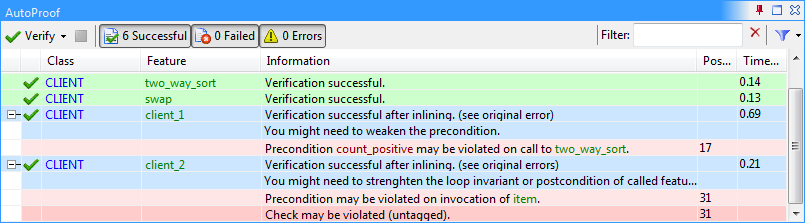
\includegraphics[width=\columnwidth]{images/eve_panel_twostep.png}
\caption{\AutoProof showing feedback of two-step verification.}
\label{fig:two-step-feedback}
\end{figure}


Routine \e{client_2} calls \e{two_way_sort} on a four-element array and checks that its first element is \e{False} after the call.
Modular verification cannot prove this assertion: \e{two_way_sort} has no postcondition, and hence its effects within \e{client_2} are undefined.
The second verification attempt inlines \e{two_way_sort} and unrolls the loop four times (since it notices that the call is on a four-element array); this proves that the first array element is \e{False} after the call (first line in Table~\ref{tab:two-step-unroll-summary}).
In all, \e{two_way_sort} is not to blame because its implementation works correctly for \e{client_2}.
As summarized in the second line of Table~\ref{tab:two-step-inline-summary}, the user can either just be happy with the result or endeavor to write down a suitable postcondition for \e{two_way_sort} so that the correctness proof can be generalized to arrays of arbitrary length.

Suppose we provide a postcondition that specifies sortedness using Eiffel's across syntax:
\begin{erunning}
across 1..(a.count-1) as k all
				(a[k] = a[k+1]) or (a[k] /= a[k+1] and a[k] = False)
\end{erunning}
Modular verification of \e{two_way_sort} fails to prove this postcondition because the loop invariant at line~\ref{l:loop-inv} does not say anything about the array content.
Two-step verification makes a second attempt where it unrolls the loop a finite number of times, say 5, and inlines \e{swap}.
The situation is in the second entry of Table~\ref{tab:two-step-unroll-summary}: we cannot verify that the arbitrary bound of five iterations generally holds (that is $j - i + 1 \leq 5$ holds before the loop), but the success of unrolling in this limited case suggests that \e{two_way_sort}'s implementation is correct.
If we want to get to a general proof, we should improve the loop invariant, and this is precisely the suggestion that two-step verification brings forward.



%============================================================================
\subsection{Evaluation}\label{evaluation}
%============================================================================

The examples of the previous sections have demonstrated the kind of feedback two-step verification provides.
This section contains a preliminary evaluation of the scalability of two-step verification, and of its benefits in terms of reduced annotation burden.

\begin{table}[ht]
\footnotesize
\setlength{\tabcolsep}{3.8pt}
\centering 
\begin{tabular}{ r l r| rrrr r r@{.}l | rrrr r r@{.}l |}
& & & \multicolumn{7}{c|}{\textsc{two-step}} &  \multicolumn{7}{c|}{\textsc{modular}} \\
& & & {\scriptsize $P$} & {\scriptsize $Q$} & {\scriptsize $I$} & {\scriptsize $A$} & & \multicolumn{2}{c|}{} & {\scriptsize $P$} & {\scriptsize $Q$} & {\scriptsize $I$} & {\scriptsize $A$} & \multicolumn{3}{c|}{} \\[-2pt]
& & \textit{code} & \multicolumn{4}{c}{\textit{spec}} & \textit{Boogie} & \multicolumn{2}{c|}{\textit{time}} & \multicolumn{4}{c}{\textit{spec}} & \textit{Boogie} & \multicolumn{2}{c|}{\textit{time}} \\
\hline
   &          &    &  {\scriptsize 1} & {\scriptsize 3} & {\scriptsize 0} & {\scriptsize 0}   & \multicolumn{3}{c|}{} &  {\scriptsize 1} & {\scriptsize 3} & {\scriptsize 4} & {\scriptsize 0} & \multicolumn{3}{c|}{} \\[-3pt]
1. & Maximum  & 32 & \multicolumn{4}{c}{\ 4} & 1541 \ & 2&06 & \multicolumn{4}{c}{\ 8} & 712 \ & 1&05 \\
   &          &    &  {\scriptsize 3} & {\scriptsize 1} & {\scriptsize 0} & {\scriptsize 0}   & \multicolumn{3}{c|}{} &  {\scriptsize 3} & {\scriptsize 1} & {\scriptsize 5} & {\scriptsize 0} & \multicolumn{3}{c|}{} \\[-3pt]
2. & Sum and Max  & 32 & \multicolumn{4}{c}{\ 4} & 1619 \ & 2&18 & \multicolumn{4}{c}{\ 9} & 720 \ & 1&04 \\
   &          &    &  {\scriptsize 2} & {\scriptsize 1} & {\scriptsize 0} & {\scriptsize 0}   & \multicolumn{3}{c|}{} &  {\scriptsize 2} & {\scriptsize 1} & {\scriptsize 5} & {\scriptsize 0} & \multicolumn{3}{c|}{} \\[-3pt]
3. & Two-way Sort  & 44 & \multicolumn{4}{c}{\ 3} & 1803 \ & 2&35 & \multicolumn{4}{c}{\ 8} & 742 \ & 1&06 \\
   &          &    &  {\scriptsize 2} & {\scriptsize 1} & {\scriptsize 0} & {\scriptsize 0}   & \multicolumn{3}{c|}{} &  {\scriptsize 2} & {\scriptsize 1} & {\scriptsize 10} & {\scriptsize 0} & \multicolumn{3}{c|}{} \\[-3pt]
4. & Dutch Flag  & 45 & \multicolumn{4}{c}{\ 3} & 1955 \ & 2&94 & \multicolumn{4}{c}{\ 13} & 786 \ & 1&14 \\
   &          &    &  {\scriptsize 3} & {\scriptsize 4} & {\scriptsize 0} & {\scriptsize 0}   & \multicolumn{3}{c|}{} &  {\scriptsize 3} & {\scriptsize 4} & {\scriptsize 7} & {\scriptsize 0} & \multicolumn{3}{c|}{} \\[-3pt]
5. & LCP  & 30 & \multicolumn{4}{c}{\ 7} & 1585 \ & 2&10 & \multicolumn{4}{c}{\ 14} & 730\ & 1&05 \\
\hline
   &          &    &  {\scriptsize 0} & {\scriptsize 0} & {\scriptsize 0} & {\scriptsize 7}   & \multicolumn{3}{c|}{} &  {\scriptsize 5} & {\scriptsize 13} & {\scriptsize 5} & {\scriptsize 7} & \multicolumn{3}{c|}{} \\[-3pt]
6. & Priority queue & 119 & \multicolumn{4}{c}{\ 7} & 2896 \ & 3&35 & \multicolumn{4}{c}{\ 30} & 1088 \ & 1&56 \\
   &          &    &  {\scriptsize 0} & {\scriptsize 0} & {\scriptsize 0} & {\scriptsize 11}   & \multicolumn{3}{c|}{} &  {\scriptsize 7} & {\scriptsize 18} & {\scriptsize 4} & {\scriptsize 11} & \multicolumn{3}{c|}{} \\[-3pt]
7. & Deque & 127 & \multicolumn{4}{c}{\ 11} & 1856 \ & 2&51 & \multicolumn{4}{c}{\ 40} & 1230 \ & 1&59 \\
   &          &    &  {\scriptsize 0} & {\scriptsize 0} & {\scriptsize 0} & {\scriptsize 1}   & \multicolumn{3}{c|}{} &  {\scriptsize 2} & {\scriptsize 3} & {\scriptsize 0} & {\scriptsize 1} & \multicolumn{3}{c|}{} \\[-3pt]
8. & Binary Search  & 48 & \multicolumn{4}{c}{\ 1} & 2479 \ & 3&21 & \multicolumn{4}{c}{\ 6} & 672 \ & 0&99 \\
\hline \hline
   &          &    &  {\scriptsize \textit{11}} & {\scriptsize \textit{10}} & {\scriptsize \textit{0}} & {\scriptsize \textit{19}}   & \multicolumn{3}{c|}{} &  {\scriptsize \textit{25}} & {\scriptsize \textit{44}} & {\scriptsize \textit{40}} & {\scriptsize \textit{19}} & \multicolumn{3}{c|}{} \\[-3pt]
& \textit{Total} & \textit{477} & \multicolumn{4}{c}{\ \textit{40}} & \textit{15734} \ & \textit{20}&\textit{70} & \multicolumn{4}{c}{\ \textit{128}} & \textit{6680} \ & \textit{9}&\textit{48}
\end{tabular}
\caption{Comparison of two-step and modular verification on selected examples.}
\label{tab:two-step:examples}
\end{table}


Table~\ref{tab:two-step:examples} lists the example programs.
The first labeled column after the program name contains the size of the implementation (not counting specification elements) in lines of code.
The rest of the table is split in two parts: the first one contains data about two-step verification; the second one the same data about modular verification.
The data reported includes: the amount of specification necessary to successfully verify the example (number of annotations, split into preconditions $P$, postconditions $Q$, invariants $I$ (loop invariants in examples 1--5; class invariants in examples 6--8), and intermediate assertions $A$); the size (in lines) of the Boogie code generated by AutoProof; and the time in seconds.
Two-step verification includes modular verification as first step, but normally requires less specification to be successful; correspondingly, the Boogie code and the time in the first part of the table sum up both steps.
 


The examples include: 
(1)~finding the maximum in an array, from the COST 2011 verification competition~\cite{BORMER11};
(2)~computing maximum and sum of the elements in an array, from the VSTTE 2010 verification competition~\cite{KLEBANOV11};
(3)~the two-way sort algorithm of Section~\ref{sec:ap-overview}, from the VSTTE 2012 verification competition~\cite{FILLIATRE12};
(4)~Dikstra's Dutch national flag algorithm~\cite{DIJKSTRA76};
(5)~computing the longest common prefix of two sequences, from the FM 2012 verification competition~\cite{HUISMAN12};
(6)~a priority queue implementation, from Tinelli's verification course~\cite{TINELLI2011}; 
(7)~a double-ended queue~\cite[Vol.~1, Sec.~2.2.1]{KNUTH11}; and
(8)~the binary search algorithm of Section~\ref{sec:ap-overview}, from the software verification benchmarks~\cite{VSI08}. 




In the experiments with the algorithms 1--5, two-step verification succeeds with loop unrolling of depth $n=6$, which corresponds to input arrays of the same length.
The outcome suggests either to use the unrolled loop, for inputs of bounded length; or to write a suitable loop invariant.
A correct loop invariant is necessary for modular verification alone to succeed, in which case the proof generalizes to arrays of arbitrary length.
We prove the following postconditions: (1) the output is the array maximum; (2) the output sum is less than or equal to the output maximum times the array length; (3) sortedness of the output, as formalized in Section~\ref{sec:examples-two-step}; (4) the output is partitioned in the three flag colors; (5) the output is the longest common prefix of the input array.



In the experiments 6--8 we verify \emph{clients} of the queue, double-ended queue, and binary search, which call some routines and then formalize their expectations on the result with \e{assert}s after the call.
The called routines have no specification (in particular, no postcondition); two-step verification verifies the clients using inlining of the callee, and suggests to add postconditions to generalize the proofs.
The postconditions are necessary for modular verification alone to succeed.

The evaluation suggests that two-step verification can check the implementation even when little or no specification is given; its feedback may then help write the necessary specifications to generalize proofs for modular verification.


The runtime overhead of performing two verification steps instead of one is roughly linear in all examples; in fact, unrolling and inlining blow up mainly in the presence of recursion.
To better assess how they scale, we have repeated two-step verification of examples 3 (using unrolling) and 6 (using inlining in the presence of recursion) for increasing value of the bound $n$.
Table~\ref{tab:two-step:blowup} shows the results in terms of size of the generated Boogie code (in lines) and time necessary to verify it (in seconds).
Unrolling scales gracefully until about $n=10$; afterward, the time taken by Boogie to verify increases very quickly, even if the size of the Boogie code does not blow up.
Inlining is more sensitive to the bound, since the size of the inlined code grows exponentially due to the conditional branch in \e{binary_search}'s body; the time is acceptable until about $n = 7$.
Notice that the heuristics for the choice of $n$ discussed in Section~\ref{sec:bounds} would generate running times in the order of tens of seconds, thus enforcing a reasonable responsiveness.



\begin{table}[th]
\centering 
\begin{tabular}{r| r r@{.}l | r r@{.}l }
	&
	\multicolumn{3}{c|}{\textsc{unrolling}}
	&
	\multicolumn{3}{c}{\textsc{inlining}}
	\\
	\textit{inlining/unrolling depth} $n$ &
	\textit{Boogie} 
	&
	\multicolumn{2}{c|}{\textit{time}}
	&
	\textit{Boogie} 
	&
	\multicolumn{2}{c}{\textit{time}}
	\\
  \hline
 3 & 864 & 1&07 & 1201 & 1&44 \\
 4 & 937 & 1&13 & 1822 & 2&26 \\
 5 & 1010 & 1&21 & 3054 & 4&23 \\
 6 & 1083 & 1&32 & 5518 & 10&93 \\
 7 & 1156 & 1&52 & 10446 & 30&64 \\
 8 & 1229 & 2&03 & 20302 & 112&32 \\
 10 & 1375 & 4&26 & \multicolumn{1}{c}{--} & \multicolumn{2}{c}{--} \\
 13 & 1594 & 37&52 & \multicolumn{1}{c}{--} & \multicolumn{2}{c}{--} \\
 15 & 1667 & 253&30 & \multicolumn{1}{c}{--} & \multicolumn{2}{c}{--}
\end{tabular}
\caption{Scalability of unrolling and inlining on examples 3 and 6 from Table~\ref{tab:two-step:examples}.}
\label{tab:two-step:blowup}
\end{table}






%============================================================================
\subsection{Related Work}\label{related-work}
%============================================================================

The steadily growing interest for techniques and tools that make verification more approachable indicates how some of the most glaring hurdles to the progress of formal methods lie in their applicability.
Tools such as Dafny~\cite{LEINO10}, Spec\#~\cite{BARNETT05}, VCC~\cite{COHEN09}, ESC/Java2~\cite{COK05,JAMES10}, and Why3~\cite{BOBOT11} define the state of the art in static program verification.
Their approaches rely on accurate specifications, which are not easy to write and get right.

One way to ameliorate this situation is inferring specifications automatically using static~\cite{CHANG05,KOVACS09,FURIA10} or dynamic~\cite{ERNST01,WEI11,WASYLKOVSKI11} techniques.
Specifications dynamically inferred are based on a finite number of executions, and hence may be unsound; this makes them unsuitable for use in the context of static verification.
Static techniques can infer sound specifications from the program text; these are useful to document existing implementations, to discover auxiliary assertions (such as loop invariants), or for comparison with specifications independently written, but proving an implementation correct against a specification inferred from it is mostly a vacuous exercise.

The simple implicit contracts that we use in our approach express well-formedness properties of the input program, which are tacitly assumed by programmers reasoning informally about it; therefore, there is no risk of circularity.
Some static verifiers use mathematical integers or assume purity of specification functions to have well-formedness by construction; a risk is that, when they are applied to real programming languages, the corresponding semantic gap may leave some errors go unnoticed.
ESC/Java2, for example, does not check for overflows~\cite{KINIRY06}, nor if specification expressions are executable (for example, null-dereferencing could happen when evaluating a precondition).
The Dafny verifier checks well-formedness of pre- and postconditions, and may consequently require users to add explicit contracts to satisfy well-formedness. Our implicit contracts are instead added and checked automatically, without requiring users to explicitly write them.
In this sense, they are similar to approaches such as VCC, which models the semantics of the C programming language as precisely as possible.

Besides inferring specifications, another approach to facilitate formal verification is combining complementary verification techniques.
CEGAR model-checking~\cite{BEYER07}, for example, uses model-checking exhaustive verification techniques on approximate program models, combined with a form of symbolic execution to determine whether the failed verification attempts are indicative of real implementation errors or only a figment of an imprecise abstraction.
Tools such as DSD-Crasher~\cite{CSALLNER08} and our EVE~\cite{TSCHANNEN11} integrate testing and static checking to find when the errors reported by the latter are spurious.
Collaborative verification~\cite{CHRISTAKIS12} is also based on the combination of testing and static verification, and on the explicit formalization of the restrictions of each tool used in the combination.
Two-step verification also integrates the results of different techniques, with the main purpose of improving error reporting and reducing the number of annotations needed, rather than complementing the limitations of specific techniques.

The Spec\# system includes a verification debugger~\cite{MOSKAL11} to inspect error models when verification fails; more recently, an interpreter for Boogie programs~\cite{POLIKARPOVA13} can help find the sources of failed verification attempts.
Debuggers for verification can be quite useful in practice, but achieve a lesser degree of automation than two-step verification, since users need to manually inspect and understand the error models using the debugger.


